\documentclass[a0paper]{tikzposter}

\usetheme{Steph}

% Packages
\usepackage[T1]{fontenc}
\usepackage[utf8]{inputenc}
\usepackage{natbib,mdframed,amsmath,calc,graphicx,amssymb,relsize,multirow,rotating,bm,url,multicol,array,subfigure,eurosym}
\usepackage{tikz}
\usetikzlibrary{arrows,patterns, calc, arrows.meta}
\tikzset{>={Latex[width=3mm,length=5mm]}}

\renewcommand{\rmdefault}{phv}
\renewcommand{\sfdefault}{phv} 
\renewcommand{\labelitemi}{$\bullet$}

\newcommand{\compresslist}{
    \setlength{\itemsep}{1pt}
	\setlength{\parskip}{0pt}
	\setlength{\parsep}{0pt}
}

\definecolor{IGNVert}{RGB}{163, 210,  11}
\definecolor{IGNGris}{RGB}{159, 164, 168}
\definecolor{IGNGrisFonce}{RGB}{101, 105, 110}

\graphicspath{./images}


\title{\textbf{The SubDense project}}
\author{Mouhamadou Ndim, Bénédicte Bucher, Ana-Maria Raymond, Juste Raimbault, Julien Perret}
\institute{LASTIG, Univ. Gustave Eiffel, IGN-ENSG}
\titlegraphic{}

% Layout of title and logos, some other possible logos are available in images folder
% Don't hesitate to modify the positions if it doesn't suit you
\makeatletter
\renewcommand\TP@maketitle{
    \hspace{-.12\textwidth}
	\begin{tabular}{lcl}
	%logo box 1
        
    	\begin{minipage}[b][.1\textheight][b]{.15\textwidth}
      
        	
\includegraphics[scale=1.2]{./figures/LOGO_IGN}
          %
\includegraphics[scale=0.4]{./images/logo_ensg}
    	\end{minipage}
    	&
    	%title box
    	\begin{minipage}[b][.1\textheight][b]{.6\textwidth}

            
     
    		\centering
    		\color{titlefgcolor}
            \vspace{1cm}
    		{\bfseries \Huge \sc \@title \par}
    		
    		{\bfseries \huge \sc Collaborative dashboard to study periurban densification \par}
    		\vspace*{2em}
    		{\huge \@author \par}
    		\vspace*{1em}
    		{\LARGE \@institute}
    		
    	\end{minipage}
    	&
    	%logo box 2
    	\begin{minipage}[b][.1\textheight][b]{.15\textwidth}
            	
\includegraphics[width=1\textwidth]{./figures/Logo_Subdense}
    	\end{minipage}
	\end{tabular}
}
\makeatother

%%%%%%%%%%%%%%%%%%%%%%%%%%%%%%%%%%%%%%%%%%%%%%%%%%%%%%%%%%%%%%%%%%%%%%%%%%%%%%%%
% Multicol Settings
%%%%%%%%%%%%%%%%%%%%%%%%%%%%%%%%%%%%%%%%%%%%%%%%%%%%%%%%%%%%%%%%%%%%%%%%%%%%%%%%
\setlength{\columnsep}{1.5em}
\setlength{\columnseprule}{0mm}

%%%%%%%%%%%%%%%%%%%%%%%%%%%%%%%%%%%%%%%%%%%%%%%%%%%%%%%%%%%%%%%%%%%%%%%%%%%%%%%%
% Save space in lists. Use this after the opening of the list
%%%%%%%%%%%%%%%%%%%%%%%%%%%%%%%%%%%%%%%%%%%%%%%%%%%%%%%%%%%%%%%%%%%%%%%%%%%%%%%%


% To remove the "latex tikz poster" at the bottom right corner
\tikzposterlatexaffectionproofoff

\begin{document}
	% Title block with title, author, logo, etc.
	\maketitle
	
%------------------------------------------------------
%----------------LINE 1--------------------------------
%------------------------------------------------------
	\begin{columns}
		
		% first column with relative width
		% be sure that on a same line column widths sum to 1, otherwise columns are left aligned and it is awful
		
		\column{0.33}% Width set relative to text width
		
		% This is a block
		% The size of the block-title is specified with "titlewidthscale" and the name of the block is given after
		% The full formalism is \block[options]{title}{content}
		
		%==============================================
		\block[titlewidthscale=0.35]{Context}{

            \vspace{1cm}
            
			\begin{itemize}
				\item Suburban densification as a tool for more sustainable cities while avoiding many negative externalities linked to center densification (scarcity of space, price increase, housing shortage) \cite{jehling2020densification}
                \vspace{0.5cm}
				\item Multiple rationalities / conception of space of involved stakeholders (landowners, policy makers, inhabitants) coexist \cite{hartmann2019diversity}
                \vspace{0.5cm}
                \item Considerable planning challenges in associated incremental development, need for new policy insights and frameworks \cite{dunnning2020planning}
			\end{itemize}
		}
		%==============================================
		
		% Second column on same line than first one
		\column{0.34}
	    %==============================================
		\block[titlewidthscale=0.7]{The SubDense project}{

            % This project seeks to better understand the polyrationalities of space, actors and policies on suburban densification. It will explore how diverse strategies of land policy interact with landowners’ and local stakeholders’ interest and agency to shape suburban densification and their impact on suburbia across different planning systems. 
            % Thisprojectaims to addressthis knowledge gap using an innovative combination of geodata analysis with social and policy science and planning. The main research objective is to understand polyrationalities of space, actors, and policies on suburban densification. 

            The \textbf{SubDense} European project aims at better understanding \textbf{the polyrationalities of space, actors and policies on suburban densification}, by

            \bigskip

            $\rightarrow$ exploring how diverse strategies of land policy interact with landowners' and local stakeholders' interest and agency to shape suburban densification and their impact on suburbia across different planning systems (France, Germany, UK);

            \bigskip

            $\rightarrow$ combining quantitative approaches (geodata analysis and geosimulation) with qualitative approaches (social and policy science and planning).
            
		
		}
		%==============================================
		
		% Third column on first line
		\column{0.33}% Width set relative to text width
		%==============================================
		\block[titlewidthscale=0.7]{Work packages}{

            % Which data, information infrastructures and approaches enable a comparative spatial analysis of suburban densification and allow for an integration of landowners’ and local stakeholders’ interests and agency? (--> WP1)●How can landowners’ and local stakeholders’ interests and agency be explained in relation to land policies for suburban densification? (--> WP2) ●How do land policies respond to the interests and agency of landowners and local stakeholders in an effective and efficient way?  (--> WP3)
  
			\begin{itemize}
				\item \textbf{WP1:} Which data, information infrastructures and approaches enable a comparative spatial analysis of suburban densification and allow for an integration of stakeholders' interests and agency?
    
    $\rightarrow$ \textbf{main LASTIG contribution: } data integration, collaboration in data analysis, geosimulation.
				\item \textbf{WP2:} How can stakeholders' interests and agency be explained in relation to land policies for suburban densification?
                \item \textbf{WP3:} How do land policies respond to the interests and agency of stakeholders in an effective and efficient way?
			\end{itemize}
		}
		%==============================================
		%end of first line
	\end{columns}
	
%------------------------------------------------------
%----------------LINE 2--------------------------------
%------------------------------------------------------

	\begin{columns}
		
		\column{0.49}
		%==============================================
		\block[titlewidthscale=0.7]{Data expertise and analysis}{

            \begin{center}
            \includegraphics[width=0.5\linewidth]{figures/building_evolution.png}
            \hspace{2cm}
            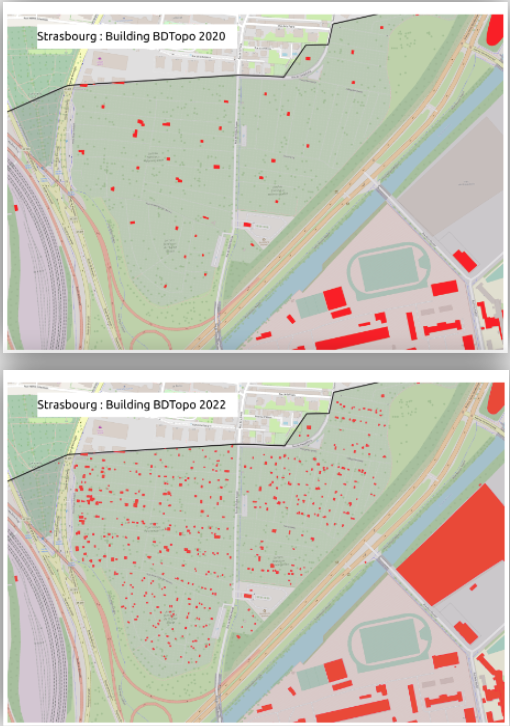
\includegraphics[width=0.25\linewidth]{figures/compar_bdtopo.png}
            \end{center}
            
            \bigskip

            $\rightarrow$ how to share analysis and methods for reproduction on other case studies (\textit{Left figure}: example of change analysis)

            \bigskip
            
            % how to integrate this knowledge on data specification into the dashboard so that it is discoverable and reusable by partners?

            $\rightarrow$ how to integrate knowledge on data specification (\textit{Right figure}: change in specifications of BDTopo 2020-2022) so that partners' analysis are not biased?
   
		}
		
		\column{0.49}
		%==============================================
		\block[titlewidthscale=0.9]{Matching algorithms for change detection}{

            \parbox{0.75\linewidth}{
              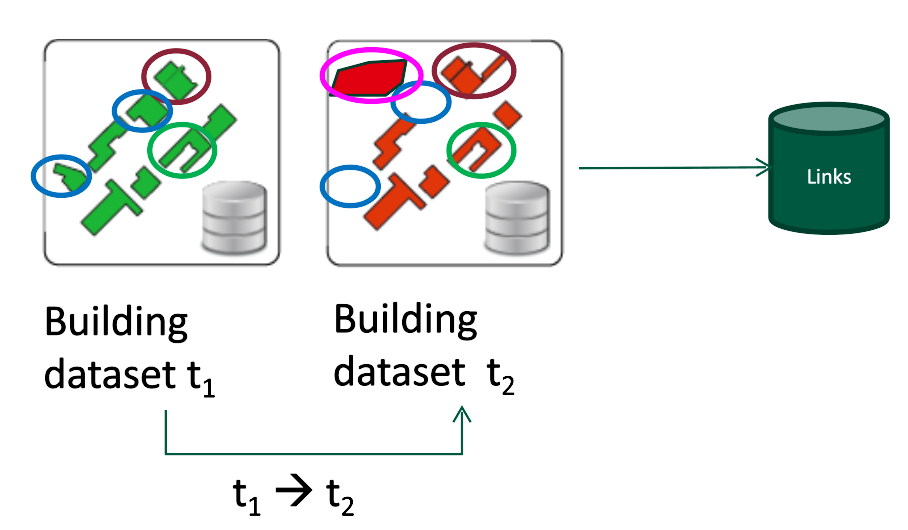
\includegraphics[width=\linewidth]{figures/matching}
		      }
            \hspace{0.5cm}
            \parbox{0.2\linewidth}{
			    \textbf{Typology of changes}

                \bigskip

                {\textcolor{green!50!black}{1:1 stability}}

                {\textcolor{blue}{1:0 destruction}}

                {\textcolor{magenta}{0:1 construction}}
		      }
  
            \vspace{2cm}

            $\rightarrow$ Benchmark of polygon matching algorithms \cite{olteanu2015knowledge}, to provide tools for building change detection

            
   
		}
		%==============================================
		
		
	\end{columns}
	
%------------------------------------------------------
%----------------LINE 3--------------------------------
%------------------------------------------------------

	% block alone on its line so you don't have to specify the columns environment

	%==============================================
	\block[titlewidthscale=0.25]{Collaborative dashboard}{
		\parbox{0.6\textwidth}{
			\begin{mdframed}
                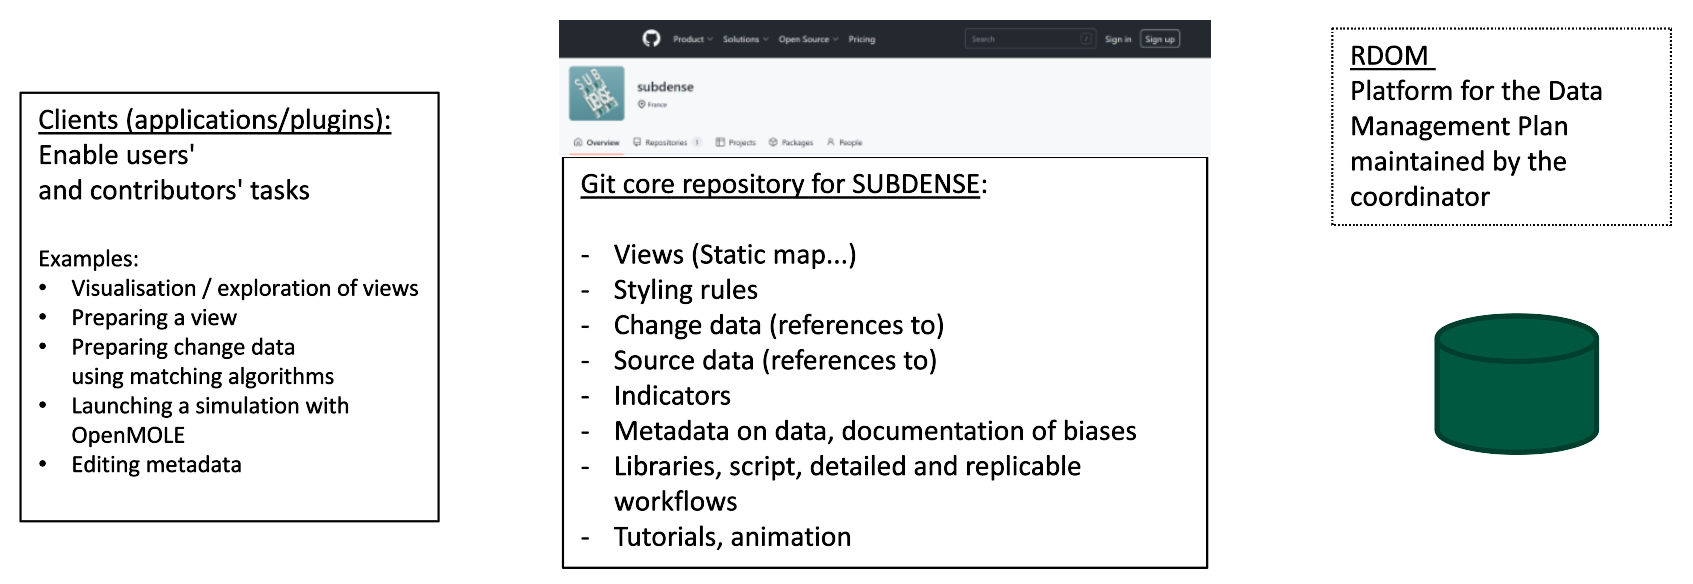
\includegraphics[width=\linewidth]{figures/dashboard_archi.png}
		      \end{mdframed}
        }
        \hspace{1cm}
		\parbox{0.3\textwidth}{
            
            $\rightarrow$ A \textbf{collaborative dashboard} as a medium to \textbf{facilitate collaboration} between partners, \textbf{share methods and data}, and ensure reproducibility 

            \bigskip
              
              % Ensures trackability, full history, reproducibility, flexibility
              % Ensure collaboration 
			$\rightarrow$ The \textbf{git-based architecture} for the core dashboard ensures tractability, full history, reproducibility, flexibility, and collaboration through branching, shared remote repository.

            \bigskip
    
            $\rightarrow$ Clients will implement interactions with the core and functionalities needed by partners for data analysis and integration (running change detection algorithms, adding data, exploring results and maps, \ldots).

            % Implementation: from user stories to dashboard specifications
            %     We propose an iterative process: progressive refinement of user stories and associated specifications​
            %List of dashboard clients/functionalities to be enriched, and discussed regarding what has priority/is feasible​
            %Architecture of the repository, ways to describe metadata, data pointers, processes, etc. and to link between all, to be defined based on user stories/practices
            %Users do not need to have git skills or contribute directly to the repository to produce user stories => shared document for these stories?
   
            \bigskip

            $\rightarrow$ An iterative process to produce \textbf{user stories}, finally leading to some specifications for the core architecture and functionalities of clients.

   
		}
		%==============================================
	}
	
%------------------------------------------------------
%----------------LINE 4--------------------------------
%------------------------------------------------------

	\begin{columns}
		%In this block you can specify possible improvment or any extra information
		\column{0.25}
		%==============================================
		\block[titlewidthscale=0.65]{Future work}{
            The second part of the project will also involve LASTIG for
			\begin{itemize}
				\item heterogeneous data integration, to couple densification analysis with socio-economic data
                \item develop and explore simulation models for the impact of policies on densification processes, parametrise these models with the qualitative data obtained through interviews during the project
			\end{itemize}
		}
		
		\column{0.25}
		%==============================================
		\block[titlewidthscale=0.6]{Project details}{
			\begin{itemize}
				\item January 2023 -- December 2025
				\item \textit{Open Research Areas} European grant: 1M\euro
				\item 4 partners institutions: TU Dortmund, IOER, University of Liverpool, IGN
                \item 8 permanent researchers, 5 short-term contracts working full time
			\end{itemize}
		}
		
		\column{0.5}
		%==============================================
		% bibliography managed with natbib
		\block[titlewidthscale=0.3,bodyoffsety=1.8cm,titleoffsety=.1cm]{References}{
			% This command is to prevent the printing of a second "références" in text and to delete white space between block title and bibliography
			\renewcommand\refname{\vskip -3.4cm}
			% Bibliography input. 
			%Refrences should be added directly to the Biblio.bib file. Refrences should in bibTex Format. Every Reference cited in the poster will be automatically added.
			
			\bibliography{Biblio}
			% Plain style so that cited articles appear as number in the poster and are only fully displayed here
			\bibliographystyle{plain}
		}
	    %==============================================	
	\end{columns}
	
\node [above right,outer sep=20pt,minimum width=\textwidth,align=center,draw=none,fill=none, text = IGNGrisFonce] at (bottomleft) {\centering \huge \bf Journées de la Recherche IGN - 2023};

\end{document}

\endinput



% Template


			\vspace{.5cm}
			
			%This block contain example of Tikz
			
			\centering
			
			\begin{tikzpicture}[scale=2]
			\draw[-latex] (0,0) -- (0,3.2);
			\draw[-latex] (0,0) -- (5.2,0);
			\node at (-0.2,1.5) {$\theta$};
			\node at (2.5,-0.2) {$\mathit{t}$};
			
			\node at (0.2,0) {$\bullet$};
			\node at (0.4,0.8) {$\bullet$};
			\node at (0.6,1.6) {$\bullet$};
			\node at (0.8,2.4) {$\bullet$};
			\node at (1.8,0.4) {$\bullet$};
			\node at (2,1.2) {\textcolor{red!60!black}{$\bullet$}};
			\node at (2.2,2) {$\bullet$};
			\node at (2.4,2.8) {$\bullet$};
			\node at (3.4,0) {$\bullet$};
			\node at (3.6,0.8) {$\bullet$};
			\node at (3.8,1.6) {$\bullet$};
			\node at (4,2.4) {$\bullet$};
			
			\draw[->,red!60!black] (2,1.2) -- (0.4,0.8);
			\draw[->,red!60!black] (2,1.2) -- (0.6,1.6);
			\draw[->,red!60!black] (2,1.2) -- (1.8,0.4);
			\draw[->,red!60!black] (2,1.2) -- (2.2,2);
			\draw[->,red!60!black] (2,1.2) -- (3.6,0.8);
			\draw[->,red!60!black] (2,1.2) -- (3.8,1.6);
			\end{tikzpicture}
			
			Exemple de Tikz 

			\vspace{.5cm}
			


